\documentclass[journal,12pt,twocolumn]{IEEEtran}

\usepackage{setspace}
\usepackage{gensymb}
\singlespacing
\usepackage[cmex10]{amsmath}

\usepackage{amsthm}

\usepackage{mathrsfs}
\usepackage{txfonts}
\usepackage{stfloats}
\usepackage{bm}
\usepackage{cite}
\usepackage{cases}
\usepackage{subfig}
\usepackage{float}
\usepackage{longtable}
\usepackage{multirow}

\usepackage{enumitem}
\usepackage{mathtools}
\usepackage{steinmetz}
\usepackage{tikz}
\usepackage{circuitikz}
\usepackage{verbatim}
\usepackage{tfrupee}
\usepackage[breaklinks=true]{hyperref}
\usepackage{graphicx}
\usepackage{tkz-euclide}

\usetikzlibrary{calc,math}
\usepackage{listings}
    \usepackage{color}                                            %%
    \usepackage{array}                                            %%
    \usepackage{longtable}                                        %%
    \usepackage{calc}                                             %%
    \usepackage{multirow}                                         %%
    \usepackage{hhline}                                           %%
    \usepackage{ifthen}                                           %%
    \usepackage{lscape}     
\usepackage{multicol}
\usepackage{chngcntr}

\DeclareMathOperator*{\Res}{Res}

\renewcommand\thesection{\arabic{section}}
\renewcommand\thesubsection{\thesection.\arabic{subsection}}
\renewcommand\thesubsubsection{\thesubsection.\arabic{subsubsection}}

\renewcommand\thesectiondis{\arabic{section}}
\renewcommand\thesubsectiondis{\thesectiondis.\arabic{subsection}}
\renewcommand\thesubsubsectiondis{\thesubsectiondis.\arabic{subsubsection}}


\hyphenation{op-tical net-works semi-conduc-tor}
\def\inputGnumericTable{}                                 %%

\lstset{
%language=C,
frame=single, 
breaklines=true,
columns=fullflexible
}
\begin{document}


\newtheorem{theorem}{Theorem}[section]
\newtheorem{problem}{Problem}
\newtheorem{proposition}{Proposition}[section]
\newtheorem{lemma}{Lemma}[section]
\newtheorem{corollary}[theorem]{Corollary}
\newtheorem{example}{Example}[section]
\newtheorem{definition}[problem]{Definition}

\newcommand{\BEQA}{\begin{eqnarray}}
\newcommand{\EEQA}{\end{eqnarray}}
\newcommand{\define}{\stackrel{\triangle}{=}}
\bibliographystyle{IEEEtran}
\raggedbottom
\setlength{\parindent}{0pt}
\providecommand{\mbf}{\mathbf}
\providecommand{\pr}[1]{\ensuremath{\Pr\left(#1\right)}}
\providecommand{\qfunc}[1]{\ensuremath{Q\left(#1\right)}}
\providecommand{\sbrak}[1]{\ensuremath{{}\left[#1\right]}}
\providecommand{\lsbrak}[1]{\ensuremath{{}\left[#1\right.}}
\providecommand{\rsbrak}[1]{\ensuremath{{}\left.#1\right]}}
\providecommand{\brak}[1]{\ensuremath{\left(#1\right)}}
\providecommand{\lbrak}[1]{\ensuremath{\left(#1\right.}}
\providecommand{\rbrak}[1]{\ensuremath{\left.#1\right)}}
\providecommand{\cbrak}[1]{\ensuremath{\left\{#1\right\}}}
\providecommand{\lcbrak}[1]{\ensuremath{\left\{#1\right.}}
\providecommand{\rcbrak}[1]{\ensuremath{\left.#1\right\}}}
\theoremstyle{remark}
\newtheorem{rem}{Remark}
\newcommand{\sgn}{\mathop{\mathrm{sgn}}}
\providecommand{\abs}[1]{\left\vert#1\right\vert}
\providecommand{\res}[1]{\Res\displaylimits_{#1}} 
\providecommand{\norm}[1]{\left\lVert#1\right\rVert}
%\providecommand{\norm}[1]{\lVert#1\rVert}
\providecommand{\mtx}[1]{\mathbf{#1}}
\providecommand{\mean}[1]{E\left[ #1 \right]}
\providecommand{\fourier}{\overset{\mathcal{F}}{ \rightleftharpoons}}
%\providecommand{\hilbert}{\overset{\mathcal{H}}{ \rightleftharpoons}}
\providecommand{\system}{\overset{\mathcal{H}}{ \longleftrightarrow}}
	%\newcommand{\solution}[2]{\textbf{Solution:}{#1}}
\newcommand{\solution}{\noindent \textbf{Solution: }}
\newcommand{\cosec}{\,\text{cosec}\,}
\providecommand{\dec}[2]{\ensuremath{\overset{#1}{\underset{#2}{\gtrless}}}}
\newcommand{\myvec}[1]{\ensuremath{\begin{pmatrix}#1\end{pmatrix}}}
\newcommand{\mydet}[1]{\ensuremath{\begin{vmatrix}#1\end{vmatrix}}}
\numberwithin{equation}{subsection}
\makeatletter
\@addtoreset{figure}{problem}
\makeatother
\let\StandardTheFigure\thefigure
\let\vec\mathbf
\renewcommand{\thefigure}{\theproblem}
\def\putbox#1#2#3{\makebox[0in][l]{\makebox[#1][l]{}\raisebox{\baselineskip}[0in][0in]{\raisebox{#2}[0in][0in]{#3}}}}
     \def\rightbox#1{\makebox[0in][r]{#1}}
     \def\centbox#1{\makebox[0in]{#1}}
     \def\topbox#1{\raisebox{-\baselineskip}[0in][0in]{#1}}
     \def\midbox#1{\raisebox{-0.5\baselineskip}[0in][0in]{#1}}
\vspace{3cm}
\title{CBSE Maths Questions 2015}
\author{RAJASEKHAR JALA }
\maketitle
\newpage
\bigskip
\renewcommand{\thefigure}{\theenumi}
\renewcommand{\thetable}{\theenumi}
%
Get latex-tikz codes from 
%
\begin{lstlisting}
https://github.com/Sekharjala/CBSE/tree/main/CBSE/CBSE2015
\end{lstlisting}
\section{Section-A}
\begin{enumerate}
\item If the quadratic equation $px^2 – 2 \sqrt{5} px + 15 = 0 $ has two equal roots,then find the value of p.
\item In Figure 1, a tower AB is 20 m high and BC, its shadow on the ground,is 203 m long. Find the Sun’s altitude.
\begin{figure}[h!]
    \centering
    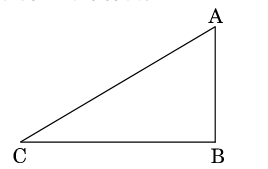
\includegraphics[width=5cm]{image1.png}
 \end{figure}
\item Two different dice are tossed together. Find the probability that the product of the two numbers on the top of the dice is 6.
\item In Figure 2, PQ is a chord of a circle with centre O and PT is a tangent. If $\angle QPT = 60 \degree,$ Find $\angle PRQ $.
 \begin{figure}[h!]
    \centering
    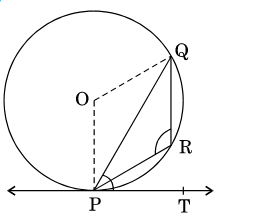
\includegraphics[width=4cm]{image2.png}
 \end{figure}
 \item In Figure 3, two tangents RQ and RP are drawn from an external point R to the circle with centre O. If $\angle PRQ = 120 \degree,$ then prove that $OR = PR + RQ $
  \begin{figure}[H]
    \centering
    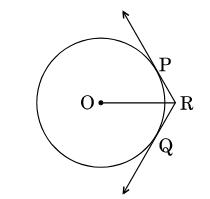
\includegraphics[width=5cm]{image3.png}
  \end{figure} 
\section{Section-B}
\item In Figure 4, a triangle ABC is drawn to circumscribe a circle of radius 3 cm, such that the segments BD and DC are respectively of lengths 6 cm  and 9 cm. If the area of $\triangle ABC is 54 cm^2,$ then find the lengths of sides AB and AC.
\begin{figure}[h!]
    \centering
    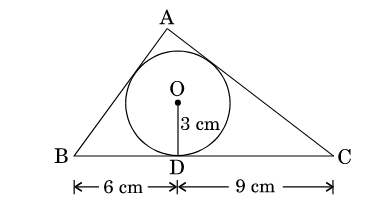
\includegraphics[width=5cm]{image4.png}
 \end{figure}
 \item Solve the following quadratic equation for x:
 \begin{center}
     $ 4x^2 + 4bx – (a^2–b^2) = 0 $
 \end{center}
 \item In an AP, if $ S_5 + S_7 = 167 $ and $S_{10}= 235,$ then find the AP, where $ S_n $ denotes the sum of its first n terms.
 \item The points $ \vec{A}= \myvec{4 & 7} $ , $ \vec{B}=\myvec{p & 3} $ and $ \vec{C}\myvec{7 & 3} $ are the vertices of a right triangle, right-angled at $ \vec{B} $. Find the value of p.
 \item Find the relation between x and y if the points $ \vec{A}=\myvec{x & y}$ ,$ \vec{B}=\myvec{-5&7} $ and $ \vec{C}=\myvec{-4&5}$ are collinear.
\section{Section C}
 \item The $14^{th}$ term of an AP is twice its $8^{th}$ term. If its $6^{th}$ term is $– 8,$ then find the sum of its first 20 terms.
\item Solve for x : \\
 \begin{center}
     $\sqrt{3}x^2 -2\sqrt{2}x-2\sqrt{3}= 0 $
 \end{center}
 \item The angle of elevation of an aeroplane from a point A on the ground is $60 \degree  $. After a flight of 15 seconds, the angle of elevation changes to $  30 \degree.$ If the aeroplane is flying at a constant height of 15003 m, find the speed of the plane in km/hr.
 \item If the coordinates of points $\vec{A}$ and $\vec{B}$ are $\myvec{– 2 &– 2}$ and $\myvec{2&–4}$ respectively, find the coordinates of P such that $AP =\frac{3}{7}$ AB, where P lies on the line segment AB.
 \item The probability of selecting a red ball at random from a jar that contains only red, blue and orange balls is $\frac{1}{4}.$ The probability of selecting a blue ball at random from the same jar is $\frac{1}{3}.$ If the jar contains 10 orange balls, find the total number of balls in the jar.
 \item Find the area of the minor segment of a circle of radius 14 cm, when its central angle is $60 \degree.$ Also find the area of the corresponding major segment. [Use $\pi =\frac{22}{7}$]
 \item Due to sudden floods, some welfare associations jointly requested the government to get 100 tents fixed immediately and offered to contribute $ 50\% $ of the cost. If the lower part of each tent is of the form of a cylinder of diameter 4.2 m and height 4 m with the conical upper part of same diameter but of height 2.8 m, and the canvas to be used $costs < 100 per sq. m,$ find the amount, the associations will have to pay. What values are shown by these associations ? [Use $\pi=\frac{22}{7}$]
 \item A hemispherical bowl of internal diameter 36 cm contains liquid. This liquid is filled into 72 cylindrical bottles of diameter 6 cm. Find the height of the each bottle, if $10 \% $ liquid is wasted in this transfer.
 \item A cubical block of side 10 cm is surmounted by a hemisphere. What is thelargest diameter that the hemisphere can have ? Find the cost of painting the total surface area of the solid so formed, at the rate of Rs. 5 per 100 sq. cm.[ Use $\pi= 3.14$ ]
\section{Section D} 
 \item 504 cones, each of diameter 3.5 cm and height 3 cm, are melted and recast into a metallic sphere. Find the diameter of the sphere and hence find its surface area. [Use $\pi=\frac{22}{7}$]
 \item The diagonal of a rectangular field is 16 metres more than the shorter side. If the longer side is 14 metres more than the shorter side, then find the lengths of the sides of the field.
 \item Find the $60^{th}$ term of the AP $8, 10, 12, ...,$ if it has a total of 60 terms and hence find the sum of its last 10 terms.
 \item A train travels at a certain average speed for a distance of 54 km and then travels a distance of 63 km at an average speed of 6 km/h more than the first speed. If it takes 3 hours to complete the total journey, what is its first speed ?
 \item Prove that the lengths of the tangents drawn from an external point to a circle are equal.
 \item Prove that the tangent drawn at the mid-point of an arc of a circle is parallel to the chord joining the end points of the arc.
 \item  Construct a $\triangle ABC $ in which $ AB = 6 cm $ , $\angle A = 30\degree $ and $\angle B = 60\degree.$ Construct another $\triangle AB'C' $ similar to $\triangle ABC $ with base $AB' = 8 cm $ .
 \item At a point A, 20 metres above the level of water in a lake, the angle of elevation of a cloud is $30 \degree.$ The angle of depression of the reflection of the cloud in the lake, at A is $60\degree .$ Find the distance of the cloud from A.
 \item A card is drawn at random from a well-shuffled deck of playing cards. Find the probability that the card drawn is
 \begin{itemize}
     \item a card of spade or an ace.
     \item a black king. 
     \item neither a jack nor a king.
     \item either a king or a queen
 \end{itemize}
 \item Find the values of k so that the area of the triangle with vertices $\myvec{1 &– 1}, \myvec{– 4 & 2k} $ and $\myvec{–k & –5}$ is 24 sq. units.
 \item In Figure 5, PQRS is a square lawn with side PQ = 42 metres. Two circular flower beds are there on the sides PS and QR with centre at O, the intersection of its diagonals. Find the total area of the two flower beds (shaded parts).
 \begin{figure}[H]
    \centering
    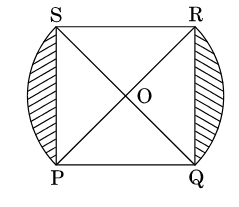
\includegraphics[width=5cm]{image5.png}
 \end{figure}
 \item Solve From each end of a solid metal cylinder, metal was scooped out in hemispherical form of same diameter. The height of the cylinder is 10 cm and its base is of radius 4.2 cm. The rest of the cylinder is melted and converted into a cylindrical wire of 1.4 cm thickness. Find the length of the wire. [Use $ \pi=\frac{22}{7} $]
  \end{enumerate}
\end{document}
